%%%%%%%%%%%%%%%%%%%%%%%%%%%%%%%%%%%%%%%%%
% Beamer Presentation
% LaTeX Template
% Version 1.0 (10/11/12)
%
% This template has been downloaded from:
% http://www.LaTeXTemplates.com
%
% License:
% CC BY-NC-SA 3.0 (http://creativecommons.org/licenses/by-nc-sa/3.0/)
%
%%%%%%%%%%%%%%%%%%%%%%%%%%%%%%%%%%%%%%%%%

%----------------------------------------------------------------------------------------
%	PACKAGES AND THEMES
%----------------------------------------------------------------------------------------

\documentclass{beamer}

\mode<presentation> {

% The Beamer class comes with a number of default slide themes
% which change the colors and layouts of slides. Below this is a list
% of all the themes, uncomment each in turn to see what they look like.

%\usetheme{default}
%\usetheme{AnnArbor}
%\usetheme{Antibes}
%\usetheme{Bergen}
%\usetheme{Berkeley}
%\usetheme{Berlin}
%\usetheme{Boadilla}
%\usetheme{CambridgeUS}
%\usetheme{Copenhagen}
%\usetheme{Darmstadt}
%\usetheme{Dresden}
%\usetheme{Frankfurt}
%\usetheme{Goettingen}
%\usetheme{Hannover}
%\usetheme{Ilmenau}
%\usetheme{JuanLesPins}
%\usetheme{Luebeck}
\usetheme{Madrid}
%\usetheme{Malmoe}
%\usetheme{Marburg}
%\usetheme{Montpellier}
%\usetheme{PaloAlto}
%\usetheme{Pittsburgh}
%\usetheme{Rochester}
%\usetheme{Singapore}
%\usetheme{Szeged}
%\usetheme{Warsaw}

% As well as themes, the Beamer class has a number of color themes
% for any slide theme. Uncomment each of these in turn to see how it
% changes the colors of your current slide theme.

%\usecolortheme{albatross}
%\usecolortheme{beaver}
%\usecolortheme{beetle}
%\usecolortheme{crane}
%\usecolortheme{dolphin}
%\usecolortheme{dove}
%\usecolortheme{fly}
%\usecolortheme{lily}
%\usecolortheme{orchid}
%\usecolortheme{rose}
%\usecolortheme{seagull}
%\usecolortheme{seahorse}
%\usecolortheme{whale}
%\usecolortheme{wolverine}

%\setbeamertemplate{footline} % To remove the footer line in all slides uncomment this line
%\setbeamertemplate{footline}[page number] % To replace the footer line in all slides with a simple slide count uncomment this line

%\setbeamertemplate{navigation symbols}{} % To remove the navigation symbols from the bottom of all slides uncomment this line
}

\usepackage{graphicx} % Allows including images
\usepackage{booktabs} % Allows the use of \toprule, \midrule and \bottomrule in tables
\usepackage{listings}
\usepackage{amsmath}
\usepackage{algpseudocode,algorithm,algorithmicx}

\lstdefinestyle{custom}{
  breaklines=true,
  frame=L,
  xleftmargin=\parindent,
  language=Java,
  showstringspaces=false,
  basicstyle=\footnotesize\ttfamily,
  keywordstyle=\ttfamily\bfseries\color{green!40!black},
  commentstyle=\ttfamily\itshape\color{gray!40!black},
  identifierstyle=\color{blue},
  stringstyle=\color{orange},
  tabsize = 2
}

%----------------------------------------------------------------------------------------
%	TITLE PAGE
%----------------------------------------------------------------------------------------

\title[Heaps]{Heaps} % The short title appears at the bottom of every slide, the full title is only on the title page

\author{Jonathan Windle} % Your name
\institute[UEA] % Your institution as it will appear on the bottom of every slide, may be shorthand to save space
{
University of East Anglia \\ % Your institution for the title page
\medskip
\textit{J.Windle@uea.ac.uk} % Your email address
}
\date{\today} % Date, can be changed to a custom date

\begin{document}

\begin{frame}
\titlepage % Print the title page as the first slide
\end{frame}

\begin{frame}[allowframebreaks]
\frametitle{Overview} % Table of contents slide, comment this block out to remove it
\tableofcontents % Throughout your presentation, if you choose to use \section{} and \subsection{} commands, these will automatically be printed on this slide as an overview of your presentation
\end{frame} 

%------------------------------------------------------------------
\section{Intro}
\begin{frame}
\frametitle{Intro}
\begin{itemize}
\item It is a {\color{red} complete binary tree}.
\item Value at each node in a (max) heap is at least as large as the value at its children nodes.
\item Let $X$ be a totally ordered set. A heap on $X$ is either empty or it is a complete binary tree, $t$, comprising $n_t \geq 1$ nodes to each node of which a value of $X$ is assignes such that:\\
value of node $i \leq$ value of parent of node $i, i = 2,3,...n_t$.
\item The {\color{green} size} of a heap is the number of nodes in the tree.
\end{itemize}
\end{frame}

%------------------------------------------------------------------
\defverbatim[colored]\sifup{
\begin{lstlisting}[style = custom]
void siftUp (Comparable [] a, int k, int m) {
// Value just added
	Comparable v = a[k];
// Index to last element
	int j = k;
// Index to parent of added element
	int i = j/2;
// While parent is greater than the element added
	while (i > 0 && a[i].compareTo(v) < 0) {
// Swap elemets around
		a[j] = a[i];
		j = i;
		i = j/2;
	}
	a[j] = v;
}
\end{lstlisting}
}
\section{Array implementation}
\begin{frame}
\frametitle{Array implementation}
\begin{itemize}
\item The root is stored in \texttt{heapArray[1]}.
\item If the value of a node, $s$, is stored in \texttt{heapArray[$i$]}, then the value of $s$ is stored in \texttt{heapArray[$2\times i$]} and the value of the right child of $s$ is stored in \texttt{heapArray[$2 \times i + 1$]}.
\end{itemize}
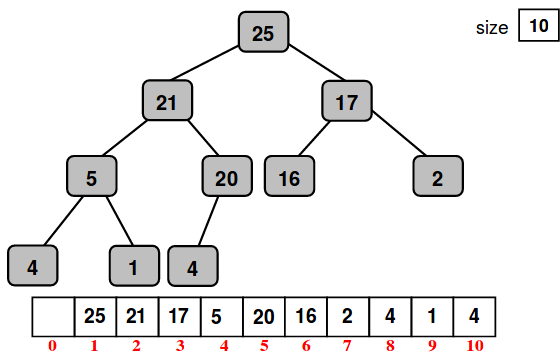
\includegraphics[scale=0.3]{array.png}
\end{frame}
%----------------------------------------------------------------
\defverbatim[colored]\sifDown{
\begin{lstlisting}[style = custom, basicstyle = \tiny]
void siftDown (Comparable [] a, int k, int m) {
// m is the size of the heap
// Start at 1
	Comparable v = a[k];
	int max_index;
	Comparable maxCh;
// i starts at 1
	int i = k;
// Determine that the node has at least on child
	boolean more = m >= 2*k;
	while(more) {
// Get position of the child that's bigger
		max_index = maxChild(a,i,m);
		maxCh = a[max_index];
// If the item is smaller than the max child, swap, otherwise stop.
		if (v.compareTo(maxCh) < 0) {
// Swap
			a[i] = maxCh;
			i = max_index;
// Determine that the node has children
			more = m >= 2*i;
		}
		else
			more = false
	}
	a[i] = v;
}
\end{lstlisting}
}
\subsection{Sift up}
\begin{frame}
\frametitle{Sift up}
\sifup
\end{frame}
%------------------------------------------------------------------
\subsection{Sift Down}
\begin{frame}
\frametitle{Sift Down}
\sifDown
\end{frame}
%---------------------------------------------------------------------
\defverbatim[colored]\del{
\begin{lstlisting}[style = custom]
void deleteMax() {
// Replace with last element added, reduce size
	heapArray[1] = heapArray[size--];
// Sift that element down to replace max to the top
	siftDown(heapArray,1,size);
}	
	
\end{lstlisting}
}

\defverbatim[colored]\insert{
\begin{lstlisting}[style = custom]
void insert(Comparable item) {
	if(size == maxSize)
		// Double array size
// increase size and add to the end of the array
	heapArray[++size] = item;
// Sift up to restore heap quality
	siftUp(heapArray,size,size);
}	
	
\end{lstlisting}
}
\subsection{Methods}
\begin{frame}
\frametitle{Methods}
\begin{itemize}
\item {\color{red}delete:}
\del
\item {\color{green} insert:}
\insert
\end{itemize}
\end{frame}

%-----------------------------------------------------------------
\subsection{Heapify}
\begin{frame}
\frametitle{Heapify}
\begin{itemize}
\item This is taking an array and turning it into a heap
\item $O(nlogn)$:
\begin{itemize}
\item Simply add all of the array elements to the \texttt{heapArr} and then iterate through calling \texttt{siftUp()} on all of them elements.
\end{itemize}
\item $O(n)$:
\begin{itemize}
\item Add all of the array elements to the \texttt{heapArr} with height of underlying tree being $l$.
\item Make each of the subtrees whose roots are at level $l - 1$ into a heap, using \texttt{siftDown()}.
\item Repeat this pocess for every subtree rooted at each previous level down to and including 0.
\end{itemize}
\end{itemize}
\end{frame}

%---------------------------------------------------------------
\section{Heap Sort}
\begin{frame}
\frametitle{Heap Sort}
\begin{itemize}
\item To sort $n$ values using \texttt{HeapSort}:
\begin{enumerate}
\item Construct a heap from the n values using the $O(n)$ {\color{green} heapify} method.
\item Output the value at the top (largest value)
\item Then \texttt{deleteMax()} to remove it.
\item Repeat step 2 until all are outputted.
\end{enumerate}
\item Run time complexity is:\\
$c_1 n + \displaystyle\sum_{i=1}^{n} ( c_2 + c_3logi)$\\
Which is $O(nlogn)$
\end{itemize}
\end{frame}
%-----------------------------------------------------------------

\begin{frame} 
\Huge{\centerline{The End}}
\end{frame}

\end{document}